\section{Durchführung}
\label{sec:durchfuehrung}
Alle Messungen werden mit einer $\SI{2}{\mega\hertz}$-Sonde durchgeführt
und mit einem bereitgestellten Programm ausgewertet.

Die ersten Messungen werden alle als Impuls-Echo-Scan durchgeführt,
als Koppelmittel wird bei allen Messungen mit den Acrylzylindern bidestilliertes
Wasser verwendet.

Zuerst wird von einem Acrylzylinder die Länge mit einer Schieblehre bestimmt,
dann werden in
einem A-Scan die Differenz zwischen den detektierten Impulsen gemessen.
Aus diesen Werten wird die Schallgeschwindigkeit in Acryl bestimmt und ins
Programm eingetragen, zur Tiefenmessung.

Für alle 7 Acrylzylindern wird ein A-Scan durchgeführt, um die Dämpfung bestimmen
zu können.
Von allen Acrylzylindern wird die Länge mit der Schieblehre bestimmt
und in der gleichen Messung wie davor, die Länge, sowie die Laufzeit bestimmt,
ebenso für zwei Kombinationen von Zylindern.

Mit einer zweiten Ultraschallsonde werden bei allen Zylindern die Laufzeiten
beim Durchschallungs-Verfahren bestimmt.

Zwei Acrylplatten und ein Zylinder mit der Länge $\SI{40}{\milli\meter}$
gestappelt, es wird eine Ultraschallsonde am Zylinder angekoppelt und eine
Messung mit 3 Peaks gespeichert.
Mit einer Fast-Fourier-Transformation wird die Frequenzverteilung bestimmt.
% Soll hier was über das Cepstrum rein?

Die letzte Messung wird an einem Augenmodell im Maßstab $1\!:\!3$, \cite{Anleitung},
durchgeführt. Mit Koppelgel wird eine Ultraschallsondean der Hornhaut angekoppelt,
vgl. Abbildung \ref{fig:augenmodell},
und die Winkelkombination gesucht, bei der die Maximale Anzahl an Peaks angezeigt wird.

\begin{figure}
    \centering
    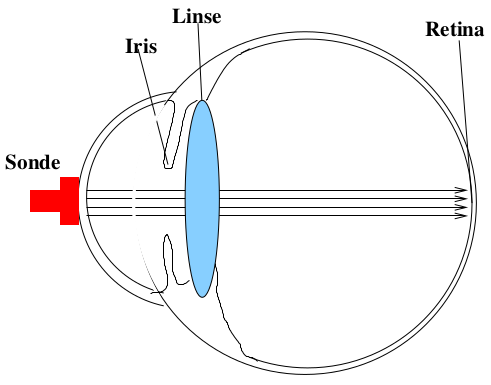
\includegraphics[width=0.5\textwidth]{content/augenmodell.png}
    \caption{Skizze des Augenmodells aus \cite{Anleitung}}
    \label{fig:augenmodell}
\end{figure}
